\begin{graphicspathcontext}{{./chapters/ai/imgs/},{./chapters/ai/imgs/auto/},\old}

\figureslide{{Data-based AI:} General Principles of Artificial Neurons}{neural_network}

\begin{frame}[t]{{Data-based AI:} Major Approaches}
	\vspace{-.4cm}
	\begin{stabularx}{X|X|X|X}
	\tabularhead{Model Type}{Key Objective}{Major Models}{Usage Examples} \\
	Supervised Learning & Predict output from labeled input & Linear Regression, SVM, Random Forest & Spam detection, price prediction \\
	\hline
	Unsupervised Learning & Discover patterns in unlabeled data & K-Means, PCA, Autoencoders & Customer segmentation, anomaly detection \\
	\hline
	Reinforcement Learning & Maximize reward through action selection & Q-Learning, DQN, PPO & Robotics, game AI, resource management \\
	\hline
	Deep Learning & Model high-dimensional data & CNN, RNN, LSTM & Image recognition, speech synthesis \\
	\hline
	Large Language Models & Generate coherent text & Transformers (Mistral, GPT) & Chatbots, translation, content creation \\
	\end{stabularx}
\end{frame}

\sidenote{Video from Linkedin}
\begin{frame}[fragile,t]{{Focus} on Large Language Models}
	\vspace{-.18cm}
	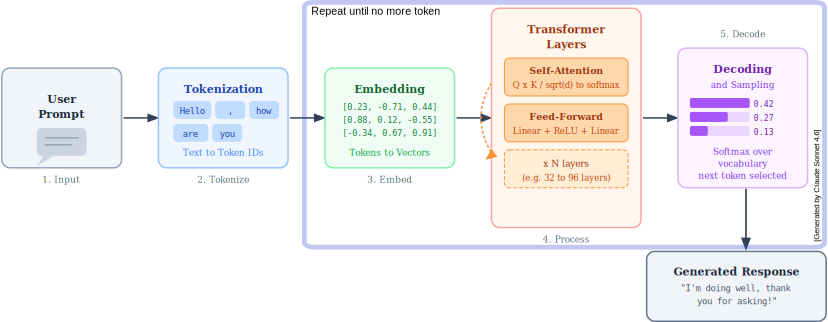
\includegraphics[width=\linewidth]{llm_process} \\
	\putat*(0,-210){\embeddedvideo[width=.5\linewidth]{./videos/ai/videollm.mp4}{videollm}}
\end{frame}

\end{graphicspathcontext}

\endinput

